

\documentclass[12pt, a4paper]{article}


\usepackage{fancyhdr, enumerate}
\usepackage{amssymb}
\usepackage{geometry, amsmath, amsfonts, float, graphicx}
\usepackage{gensymb}
\usepackage{hyperref, listings}
\usepackage{matlab-prettifier}
\usepackage{caption}
\geometry{
	top=0.9in,           
	inner=0.6in,
	outer=0.6in,
	bottom=2in,
	tmargin= 10ex,       
	headsep=0.6cm,          
}
\pagestyle{fancy}

\fancyhead{}
\fancyfoot{}

\fancyhead[L]{Bioen 316 AC \\Homework 4\\ May 1, 2019}
\fancyhead[R]{Skyler Hallinan\\ hallisky@uw.edu \\ 1732227}

\lstMakeShortInline[style=Matlab-editor]"
\begin{document}
\vspace*{-3mm}
\section*{Problem 1} 
In lecture we saw that a resistor and capacitor together act as a low-pass filter when the
input voltage is applied across the two components in series and the output voltage is
measured across the capacitor. Our derivation used the impedance divider formula,
$\mathrm{G}(\mathrm{j} \omega) \equiv V_{\mathrm{OUT}} / V_{\mathrm{IN}}=Z_{\mathrm{C}} /\left(Z_{\mathrm{C}}+Z_{\mathrm{R}}\right),$ where $V \equiv V(\mathrm{j} \omega)=\mathcal{F}\{v(t)\}$. We then determine the
magnitude and phase of the gain G(j$\omega$) at $\omega =0$, $\omega \to \infty$, and the half-power frequency.
The half-power frequency is also called the cutoff frequency $f_c$ or $\omega_c$. For an R-C circuit, $\omega_c = \frac{1}{RC}$ and $f_c= \frac{\omega_c}{2\pi}$ \\ \\
Using the technique described above, show that a resistor and inductor together act as a
low-pass filter when the input voltage is applied across the two components in series and
the output voltage is measured across the resistor. The triangle is our 0 V reference.
\begin{figure}[H]
\begin{center}
\hypertarget{plot1}{}
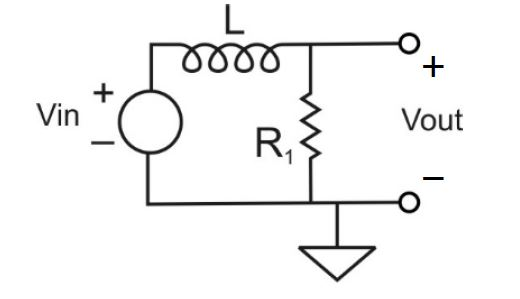
\includegraphics[width = 8cm]{fig1}
\caption{\label{fig:scaled_diss} Inductor and resistor in series to form a filter}
\end{center}
\end{figure}

\begin{enumerate}

\item Generate the complex formula for G(j$\omega$) \\ \\
\textbf{Answer: } \\
\begin{align*}
G(j\omega) &= \frac{V_{OUT}(j\omega)}{V_{IN}(j\omega)} \\
&= \frac{Z_{R1}}{Z_{R1} + Z_{C}}\\
&= \frac{R_1}{R_1 + j\omega L} &\text{Complex gain} \\
\left |  \frac{R_1}{R_1 + j\omega L} \right | &= \frac{R_1}{\sqrt{R_1^2 +( \omega L) ^2}}  &\text{Overall magnitude}
\end{align*}
\item Make the following three plots, in which $\omega$ is on a log scale.

\subitem $|G(j \omega)|$ vs. $\omega,$ where $|G(j \omega)|$ is on a linear scale from 0 to 1
\subitem $|G(j \omega)|$ vs. $\omega,$ where $|G(j \omega)|$ is on a decibel scale from 0 downward, and
\subitem $\angle \mathrm{G}(j \omega)$ vs. $\omega,$ where $\angle \mathrm{G}(\mathrm{j} \omega)$ is on a linear scale with limits of $-\pi$ and $+\pi$ \\

See attached paper for work and graphs.
\end{enumerate}
\section*{Problem 2}
The figure below shows a series RLC circuit with the output measured across the capacitor.
The diagram includes two probes (V in a circle pointing to a wire). The left probe measures
the input and the right probe measures the output voltage. Both are referenced to ground.

\begin{figure}[H]
\begin{center}
\hypertarget{plot1}{}
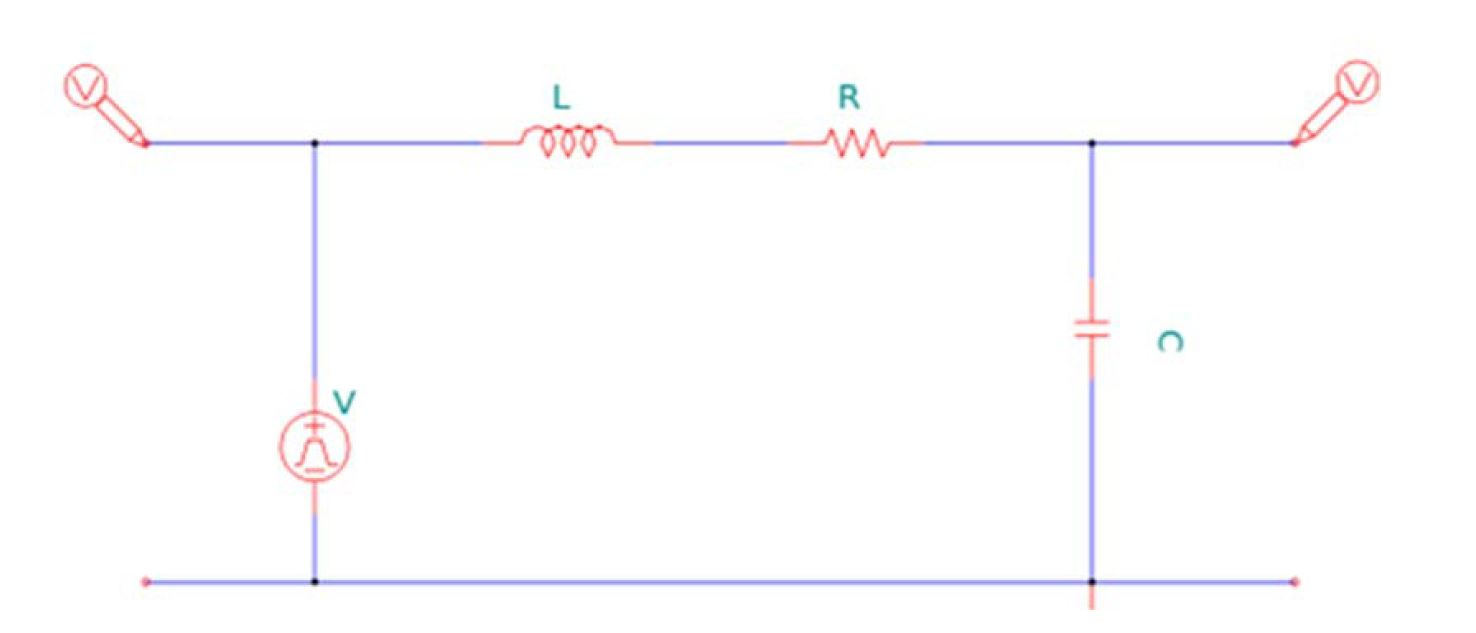
\includegraphics[width = 8cm]{fig2}
\caption{\label{fig:scaled_diss} RLC Circuit}
\end{center}
\end{figure}
\begin{enumerate}
\item Use impedances to derive the complex gain formula for this circuit, $V_C({j\omega}) / V_{IN}(j\omega)$ \\ \\
\textbf{Answer: } \\
\begin{align*}
G(j\omega) &= \frac{V_{OUT}(j\omega)}{V_{IN}(j\omega)} \\
&= \frac{Z_{C}}{Z_{R} + Z_{L}+Z_{C}}\\
&= \frac{\frac{1}{j\omega C}}{R + j\omega L + \frac{1}{j\omega C}} &\text{Complex gain} \\
&= \frac{1}{Rj\omega C - w^2 LC + 1}\ \\
\left |  \frac{1}{Rj\omega C - w^2 LC + 1} \right | &= \frac{1}{\sqrt{(R\omega C)^2 + (1-\omega^2 LC)^2}}  &\text{Overall magnitude}
\end{align*}
\item What general type of filter does this circuit provide? \\ \\
\textbf{Answer: } \\
We see that from above, we have $|G(\omega)| = \frac{1}{\sqrt{(R\omega C)^2 + (1-\omega^2 LC)^2}}$. Therefore as $\omega \to \infty$, $|G(\omega)| \to 0$, and as $\omega \to 0$, $|G(\omega)| \to \infty$. Therefore this is a low pass filter; as the frequency $\omega$ incresaes, the gain decreases, which means that lowr frequency signals pass through better. 
\item Assume that $R=5.1 \mathrm{k} \Omega, L=100 \mathrm{mH},$ and $C=33 \mu \mathrm{F}$ . At what frequency does $G(j\omega)$ become completely imaginary? \\ \\
\textbf{Answer: } \\
We have the following knowns: 
\begin{align*}
G(j\omega) = \frac{1}{Rj\omega C - w^2 LC + 1}, R = 51,000 \Omega, L = 0.1 H, C = 0.000033 F
\end{align*}
Then we substitute into our complex equation
\begin{align*}
G(j\omega) &= \frac{1}{(51,000 \cdot 0.000033 \cdot \omega j) - (w^2 \cdot 0. 1 \cdot 0.000033) + 1} \\
&= \frac{1}{1.683 j \omega - 3.3 \times 10^{-6} \omega + 1}
\end{align*}
We see that we have real and imaginary parts in the denominator. In order for the complex gain to be completely imaginary, the real parts must cancel out, leaving only the imaginary part. Thus we create the equation:
\begin{align*}
-3.3\times 10^{-6} \omega ^2 &= 1 \\
\omega &= 550.482 &\text{Ignore negative frequency}\\
G(550.482 j) &= \frac{1}{1.683 \cdot 550.482 \cdot j} &\text{Imaginary}
\end{align*}
Thus we see that with an $\omega$ of 550.482 rads/s, we achieve a completely imaginary complex gain.
\end{enumerate}
\pagebreak
\end{document}